\documentclass[conference]{IEEEtran}
\IEEEoverridecommandlockouts
% The preceding line is only needed to identify funding in the first footnote. If that is unneeded, please comment it out.
\usepackage{cite}
\usepackage{amsmath,amssymb,amsfonts}
\usepackage{algorithmic}
\usepackage{graphicx}
\usepackage{textcomp}
\usepackage{xcolor}
\def\BibTeX{{\rm B\kern-.05em{\sc i\kern-.025em b}\kern-.08em
    T\kern-.1667em\lower.7ex\hbox{E}\kern-.125emX}}
\begin{document}

\title{Conference Paper Title}
\author{
    I-Pei Lee, Chi-Hsiang Lo, \\
    \textit{Department of Electrical Engineering, National Taiwan University, Taipei, Taiwan, ROC}
}

\maketitle

\subsection{Navigation}

The navigation system is based on the ROS navigation stack \cite{navigation_stack}. Fig.~\ref{fig_navigation} shows the architecture of the navigation system. The navigation system consists of four main parts: the extended Kalman filter (EKF) \textbf{(EKF Localization)}, simultaneous localization and mapping (SLAM) \textbf{(SLAM Toolbox)}, path planning \textbf{(Global Planner)}, and local controller \textbf{(Local Controller)}.

\begin{figure}[htbp]
    \centerline{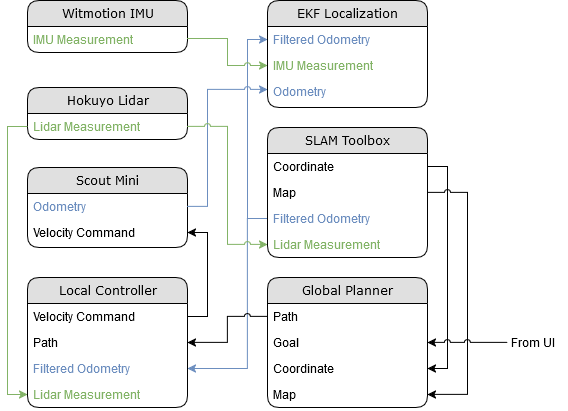
\includegraphics[width=0.5\textwidth]{figures/architecture.png}}
    \caption{Architecture of the navigation system.}
    \label{fig_navigation}
\end{figure}

\subsubsection{EKF Localization}

During development, we discovered that only relying on the Scout Mini's odometry data is not accurate enough owing to the high wheel slippage of the robot in the indoor environment, especially when the robot is turning. Hence, in order to improve the accuracy of the robot's pose estimation, we utilized \verb|robot_localization| \cite{robot_localization} ROS package to implement the EKF for localization.

By fusing an additional inertial measurement unit (IMU) that provides accurate orientation data with the odometry data that provides relative accurate translation data, the EKF can provide localization data that is accurate in both orientation and translation.

\subsubsection{SLAM}

The ROS package \verb|slam_toolbox| \cite{slam_toolbox} is selected for the SLAM algorithm over the \verb|gmapping| \cite{gmapping} package ubiquitous in ROS 1 projects. The \verb|slam_toolbox| package can also be used as a localizer without requiring additional packages such as \verb|amcl| provided by the navigation stack that is found not suitable for our inaccurate odometry system during testing, which is required by the \verb|gmapping| package in order to localize the robot in the map.

The shopping scene is first mapped and stored using \verb|slam_toolbox| as shown in Fig.~\ref{fig_map}, which is used to localize the robot for navigation tasks.

\begin{figure}[htbp]
    \centerline{
\includegraphics[width=0.5\textwidth]{figures/map.png}}
    \caption{Map of shopping scene generated by \texttt{slam\_toolbox}.}
    \label{fig_map}
\end{figure}

Here the pose estimates from the EKF are used as references for the SLAM to produce globally accurate localization data relative to the map.

\subsubsection{Global Planner}

The ROS package \verb|global_planner| provided by the navigation stack is used for path planning to generate a path from the current robot pose to the goal pose. The \verb|global_planner| package is based on the Dijkstra algorithm to generate paths that are collision-free based on the map generated by the SLAM system.

The globally accurate localization data from the SLAM is used as references for the global planner to generate a path that is accurate relative to the map.

\subsubsection{Local Controller}

The ROS package \verb|dwa_local_planner| provided by the navigation stack is used for local controller to generate velocity commands for the robot to follow the path generated by the global planner. The \verb|dwa_local_planner| package is based on the dynamic window approach (DWA) algorithm to generate velocity commands that are collision-free based on the lidar data.

The globally accurate localization data from the SLAM is not suitable for the high-frequency local controller as the localization data has lower update frequency and jumps between estimates. Hence the higher-frequency and smooth pose estimates from the EKF are used as references for the local controller to generate velocity commands.

\section{Conclusions}

In this project, we presented the design and implementation of a shopping assistance robot capable of providing various functionalities to enhance the shopping experience. The robot can navigate customers to their desired products and detect products that need restocking using the vision system, thereby maintaining inventory levels efficiently. Furthermore, the robot can transport products from the stock to the rack, streamlining the restocking process.

The entire system is controlled through a user-friendly graphical interface accessible to both customers and clerks, making it easy to interact with the robot and utilize its functionalities. The integration of these features demonstrates the potential of robotics in revolutionizing the retail industry by improving customer satisfaction and operational efficiency.

\begin{thebibliography}{00}

    \bibitem{navigation_stack} S. Macenski, F. Martín, R. White, J. Clavero. ``The Marathon 2: A Navigation System,'' IEEE/RSJ International Conference on Intelligent Robots and Systems (IROS), 2020.

    \bibitem{robot_localization} T. Moore and D. Stouch, ``A Generalized Extended Kalman Filter Implementation for the Robot Operating System,'' in Proc. 13th Int. Conf. Intell. Auton. Syst. (IAS-13), July 2014.

    \bibitem{slam_toolbox} Macenski, S., Jambrecic I., ``SLAM Toolbox: SLAM for the dynamic world,'' Journal of Open Source Software, 6(61), 2783, 2021.

    \bibitem{gmapping} Giorgio Grisetti, Cyrill Stachniss, and Wolfram Burgard, ``Improved Techniques for Grid Mapping with Rao-Blackwellized Particle Filters,'' IEEE Transactions on Robotics, Volume 23, pages 34-46, 2007.

\end{thebibliography}

\end{document}
